\section{CTR\_DRBG Counter mode Deterministic Random Bit Generator}
\label{sec:counter_mode_deterministic_random_bit_generator}

\begin{quote}
\textbf{CTR\_DRBG (Counter mode Deterministic Random Bit Generator)} is a standardized method for constructing a deterministic random bit generator (PRNG) using a block cipher operating in counter (CTR) mode. This technique is defined in NIST Special Publication 800-90A, titled \textit{``Recommendation for Random Number Generation Using Deterministic Random Bit Generators''}. Essentially, CTR\_DRBG transforms a secure symmetric cipher---such as AES---into a cryptographically strong source of pseudorandom bits. The counter mode ensures that each generated block is unique by systematically incrementing a counter value for each new data request, thus preventing the repetition of output sequences under the same key and seed. This approach is widely used in cryptographic applications requiring high security and reliability in random data generation, such as key generation, initialization vectors, and session tokens.
\end{quote}

\subsection*{How It Works}

The internal state of the CTR\_DRBG consists of two components:

\begin{itemize}
    \item \textnormal{\textbf{V}}: A state vector that acts as a counter.
    \item \textnormal{\textbf{Key}}: A symmetric encryption key (commonly 128 or 256 bits).
\end{itemize}

To generate random output, the algorithm encrypts sequential values derived from \texttt{V} using the current \texttt{Key}. For each block of output, the counter \texttt{V} is incremented. 

A secure seed—typically composed of entropy input, a nonce, and optional personalization string—is required to properly initialize the internal state.

\textit{CTR\_DRBG} utilizes an approved block cipher algorithm in counter (CTR) mode, as described in \cite{nist80090a}. Unlike the standard CTR mode, it allows the counter field to occupy only a portion of the cipher input block, as specified in \cite{nist80038d}.

For context, the block size depends on the cipher: 64 bits for TDEA and 128 bits for AES. The same block cipher algorithm and key length are used consistently throughout all encryption operations in the DRBG. These parameters must meet or exceed the required security level of the intended application.

The construction of \textit{CTR\_DRBG} revolves around an internal update function, \texttt{CTR\_DRBG\_Update}, illustrated in Figure~\ref{fig:ctr_drbg_update}. This function is invoked during instantiation, reseeding, and random bit generation to update the internal state using newly provided entropy or additional input. It also ensures that the internal state changes appropriately after every generation step.

Figure~\ref{fig:ctr_drbg_stages} outlines the full operation of \textit{CTR\_DRBG} in three stages: instantiation, generation, and reseeding.

\begin{figure}[htbp]
    \centering
    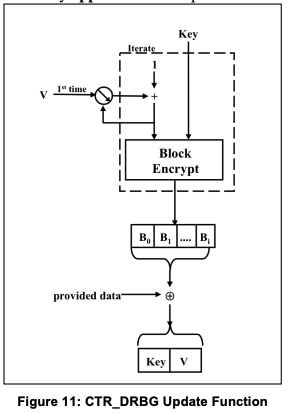
\includegraphics[width=0.9\linewidth]{images/Figure11_CTR_DRBG_Update_Function.png}
    \caption{CTR\_DRBG Update function as shown in \cite{nist80090a}.}
    \label{fig:ctr_drbg_update}
\end{figure}

\begin{figure}[htbp]
    \centering
    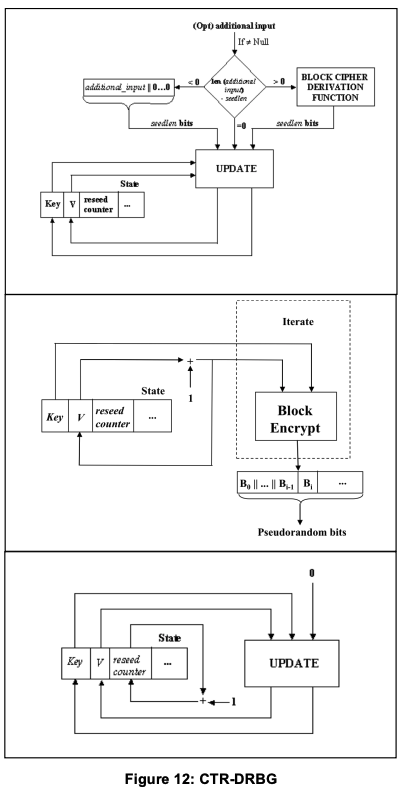
\includegraphics[width=0.9\linewidth]{images/Figure12_CTR_DRBG.png}
    \caption{The three stages of CTR\_DRBG operation as illustrated in \cite{nist80090a}.}
    \label{fig:ctr_drbg_stages}
\end{figure}

To provide an overview of what can be found in the source article, we can say that \textit{CTR\_DRBG} is a deterministic random bit generator that uses an approved symmetric encryption algorithm, such as AES, in counter (CTR) mode to produce secure random bits. Its internal state consists of a counter vector called \texttt{V} and a secret key, \texttt{Key}, which are updated through an internal function named \texttt{CTR\_DRBG\_Update} during instantiation, generation, and reseeding, thus ensuring the cryptographic security of the generator. At each step, \texttt{V} is encrypted with \texttt{Key} and incremented to generate non-repeating pseudorandom blocks. It requires a secure initial seed with sufficient entropy to avoid predictability and can be periodically reseeded to maintain long-term security. This flexible design allows for the use of variable block sizes and key lengths depending on the algorithm (e.g., 128 bits for AES) and meets robust cryptographic standards, making it reliable for applications that require secure random number generation.

\subsection{AES - Advanced Encryption Standard}
\label{sec:aes}
\begin{quote}
\textbf{AES (Advanced Encryption Standard)} is a symmetric encryption algorithm widely used across various applications for securing data. It was established by the National Institute of Standards and Technology (NIST) in 2001 as a replacement for the older Data Encryption Standard (DES). AES operates on fixed-size blocks of data (128 bits) and supports key sizes of 128, 192, or 256 bits, providing a high level of security against brute-force attacks. The algorithm employs a series of transformations, including substitution, permutation, and mixing, to encrypt plaintext into ciphertext and vice versa. Its efficiency and robustness have made it the de facto standard for encryption in many cryptographic protocols and systems.
\end{quote}
